\section{Theorie}
\label{sec:Theorie}
In diesem Versuch soll mit Hilfe eines Michelson-Interferometers die Wellenlänge $\lambda$ einer Laser-Diode bestimmt werden.
Außerdem soll der Brechungsindex $n$ von Luft ermittelt werden.
Licht ist eine Elektromagnetische Welle, welche sich im einfachsten Fall als ebene Welle der Feldstärke $\vec{E}$ darstellen lässt
\begin{equation*}
    \vec{E}(x,t)=\vec{E_0} cos(kx-\omega t - \delta) \, .
\end{equation*}
Dabei ist $k=\frac{2 \pi}{\lambda}$ die Wellenzahl, $\omega$ die Kreisfrequenz und $\delta$ ein beliebiger Phasenwikel.
Für die Lichtwellen gilt das Prinzip der linearen Superpostion, welches sich nicht überprüfen lässt, da nur die Intensität $I$ gemessen werden kann.
Da die Proportionalität $I \propto |\vec{E}|^2$ besteht, ergibt sich für die Addition von zwei Wellen
\begin{equation}
    I_\text{ges} \propto 2 \vec{E_0^2} (1+cos(\delta_2 - \delta_1)) \, .
    \label{eqn:intersch}
\end{equation}
Dabei wird deutlich das es durch den Cosinus-Term zu Interferenzerscheinungen kommt, welche von den Phasen $\delta_{1,2}$ der einzelnen Wellen abhängt.
Die Intensität verschwindet komplett, wenn die Phasendifferenz
\begin{equation*}
    \delta_2-\delta_1 = (2n+1)\pi \qquad n=0,1,2,3, ...
\end{equation*}
ist. 
Interferenzerscheinungen treten normalerweise nicht bei der Überlagerung des Lichtes von zwei unabhängigen Quellen auf, da bei allen konventionellen Lichtquellen die Phasen 
$\delta_1$ und $\delta_2$ Funktionen der Zeit sind. Dadurch verschwindet der Interfernzterm bei der Mittelung über einen Zeitraum (Groß gegenüber $\frac{2\pi}{\omega})$.
Die Ursache der Phasenfluktuation liegt im Entstehungsmechanismus des Lichtes, auf den hier nicht genauer eingegangen wird.
Kohärentes Licht, welches zum Beispiel durch Laser erzeugt werden kann, hat feste Werte für $k$, $\omega$ und $\delta$, so dass Interferenzerscheinungen gemäß Gleichung \eqref{eqn:intersch} entstehen.
Um Licht aus ein und derselben Quelle zu Überlagern werden deren Strahlen zerteilt. Dazu kann entweder ein Strahlteiler oder eine Doppelblende, wie in Abbildung \ref{fig:dopl} zu sehen, verwendet werden.
\begin{figure}
    \centering
    \caption{Prinzpielle Versuchsanordnung zur erzeugung von Interferzerscheinungen \cite{v401}}
    \label{fig:dopl}
    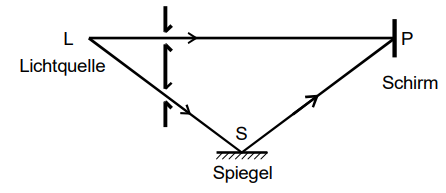
\includegraphics[width = 0.5 \textwidth]{pics/Aufbau Doppelspalt.png}
\end{figure}
Mit einem geeignetem Spiegelsystem werden die geteilten Strahlen in einem Punkt P zusammengeführt. Im allgemeinen entsteht ein Wegunterschied, wodurch eine Phasendifferenz folgt die zu Interferenz führt.
Ist dieser Wegunterschied jedoch größer als die länge der Lichtzüge, kommt es nicht mehr zu Interferenzerscheinungen, da die Lichtstrahlen zu verschiedenen Zeiten im Punkt P ankommen.
Die Kohärenzlänge $l$ ist genau die Länge, bei der im Punkt P die Interferzeffekte verschwinden.
Sie wird bestimmt über die maximal beobachtbaren Intensitätsmaxima N im Punkt P und der Wellenlänge 
\begin{equation*}
    l=N \lambda \, .
\end{equation*}
\subsection{Das Michelson-Interferometer}
Der Prinzipielle Aufbau des Michelson-Interferometers ist in Abbildung \ref{fig:mi} zu sehen.
\begin{figure}
    \centering
    \caption{prinzipieller Aufbau eines Michelson-Interferometers \cite{v401}}
    \label{fig:mi}
    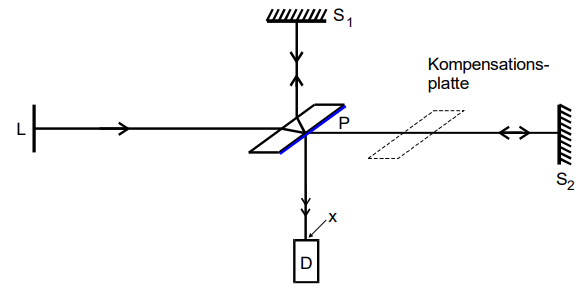
\includegraphics[width = 0.5 \textwidth]{pics/michelsoi.png}
\end{figure}
Die Lichtquelle ist am Ort L und emittiert Licht in Richtung einer pemeablen Platte P, an der die Strahlteilung erfolgt.
Teile des Lichtes fallen senkrecht auf die Spiegelflächen $S_1$ und $S_2$, wo sie zurückreflektiert werden. Die reflektierten Strahlen treffen bei P wieder zusammen und laufen parallel zueinander zum Detektor D weiter.
Die kohärenz der beiden Strahlenbündel ist gefordert, sodass der Wegunterschied nicht größer als die Kohärenzlänge werden darf. Beim verschieben von einem spiegel um die länge $\Delta d$ 
ist der Wegunterschied $2 \Delta d$. Dabei verändert sich das Interferenzmuster am Ort D. Es folgt 
\begin{equation}
    \lambda=\frac{2 \Delta d}{z} \, ,
    \label{eqn:wel}
\end{equation}
wobei z die Anzahl der beobachteten Interfernzmaxima ist. Des weiteren kann ein Wegunterschied entstehen, indem das Licht durch ein Medium der länge b mit einem Brechungsindex $n+\Delta n$ läuft.
Wenn an allen anderen Orten der Brechungsindex den Wert n hat, beträgt der Wegunterschied $\Delta n b$. Wird nun $\Delta n b$ vergrößert vom Wert null ausgehend , indem zum Beispiel der Gasdruck erhöht wird, dann verändert sich das Interferenzmuster.
Es gilt dann
\begin{equation}
    \Delta n = \frac{z \lambda}{2 b}\, ,
    \label{eqn:delt n}
\end{equation}
wobei z wieder die Anzahl der Intensitätsmaxima ist. In näherung, dass die benutzen Gase sich wie Ideale Gase in den hier verwendeten Druckbereichen verhalten, kann der Brechungsindex
$N(p_0,T_0)$ unter Normalbedingungen durch
\begin{equation*}
    N(p_0 , T_0)=1+ \Delta n \frac{T}{T_0} \frac{p_0}{p-p'} 
\end{equation*}
berechnet werden. Dabei ist $T$ die Temperatur, $p'$ der Wert vom Innendruck nach der Erniedrigung und $p$ der Wert nach der Erhöhung.
Nach einsetzen der Gleichung \eqref{eqn:delt n} folgt
\begin{equation}
    N(p_0 , T_0)=1+ \frac{z \lambda}{2 b} \frac{T}{T_0} \frac{p_0}{p-p'}  \, .
    \label{eqn:brechen}
\end{equation}

